\documentclass[0-main.tex]{subfiles}
\begin{document}


\section{Introduction}
%A large and ever increasing number of surgical procedures are performed or aided by surgical robots such as Intuitive Surgical's \textit{da Vinci}.
The prevalence of robot-assisted surgery is leading to a proliferation of datasets consisting of kinematic and fixed-camera video recordings of surgical procedures.
While these datasets have the potential to facilitate learning and autonomy, the variability of surgical data poses a unique challenge.
By nature, surgical robots interact with deformable environments and varying anatomy. 
Therefore, one of the key challenges in utilizing these datasets is to learn a common sequential structure shared across multiple instances of the same surgical task.
One model for this sequential task structure is the Transition State model~\cite{krishnan2015tsc}, which identifies spatially and temporally similar changes in motion.
Thus, while the apparent data might be highly variable, the model often learns latent similarities in tool position or kinematic state.
The learned model temporally \emph{segments} trajectories into meaningful contiguous sections, which can ultimately facilitate local learning from demonstrations, skill assessment, and salvaging good local segments from otherwise inconsistent demonstrations.

In addition to the Transition State model, there are several recent proposals to learn segmentation criteria directly from data with minimal supervision~\cite{calinon2010learning, Niekum2015learning}.
Inherently, the success of these approaches is dependent on the state representation, which is particularly challenging for visual features; especially when we want these features to perform well across different tasks. 
Inspired by the recent success of deep neural networks in reinforcement learning~\cite{levine2015end, lenz2015deep}, this paper explores how segmentation can be learned from visual state representations extracted from \textit{deep} convolutional neural networks (CNNs).

\begin{figure}[t!]
\centering
\vspace{-5pt}
% 
\includegraphics[width=0.5\linewidth]{figures/insert}
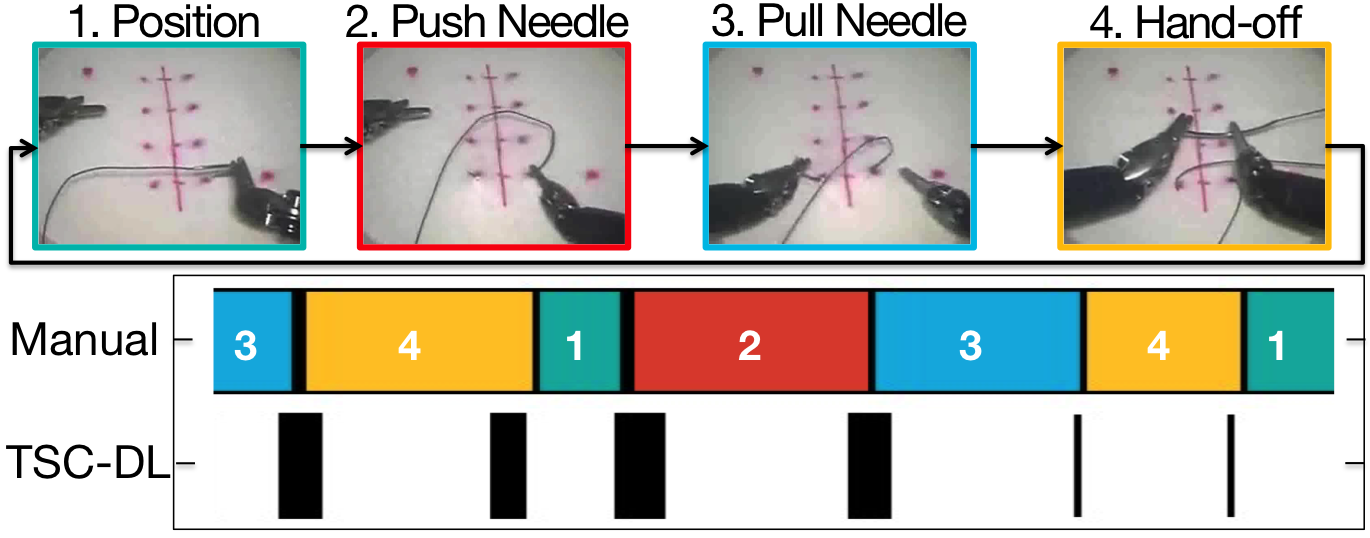
\includegraphics[width=\linewidth]{figures/suturing-teaser-v4.png}
\caption{We apply \tsc to a suturing task. Each ``throw" of suturing repeats between four steps, and figure illustrates that \tsc extracts a segmentation that closely aligns with the manual annotation without supervision.}
\figlabel{surgical-teaser}
% \label{fig:pr2_toyplane}
\vspace{-15pt} 
\end{figure}
We propose Transition State Clustering with Deep Learning (\tsc), which extends our previous work~\cite{krishnan2015tsc} with automatically constructed visual features using pre-trained CNNs.
In our prior work, we identified changes in local linearity in each trajectory, and learned a model to infer regions of the state-space at which changes occurred.
We modeled these regions as generated from a hierarchical nonparametric Bayesian model, where the number of regions are determined by a Dirichlet Process and the shape of the regions are determined by a mixture of multivariate Gaussian random variables.
Our surprising finding is that while the original Transition State model was motivated for spatial states, it empirically performs well (in comparison to ground truth) even when applied to trajectories of visual filters derived from layers of CNNs.

However, the integration of the convolutional filters with kinematics is not as straight-forward as concatenating the two parameter spaces.
This paper addresses two new issues: (1) defining metrics across multiple sensing modalities, and (2) task-trajectory correspondence.
For (1), it can be challenging to define similarity metrics across states that have both spatial and visual components.
We propose a hierarchical clustering approach that first clusters over visual space and then over kinematics, which allows us to compare kinematics-kinematics and visual-visual.  
For (2), \tsc learns a segmentation model for a task given observation of trajectories of the task.
The problem is that we may want to know how to correspond states from the individual trajectories to the segments of the task learned across all trajectories.
To learn this correspondence, we propose a novel temporal clustering technique which leverages the Jackknife estimator to correspond global segmentation structure to temporal points in the individual trajectories.




 \iffalse
\begin{SCfigure*}[][t!]
    \centering
    \vspace{-10pt}
    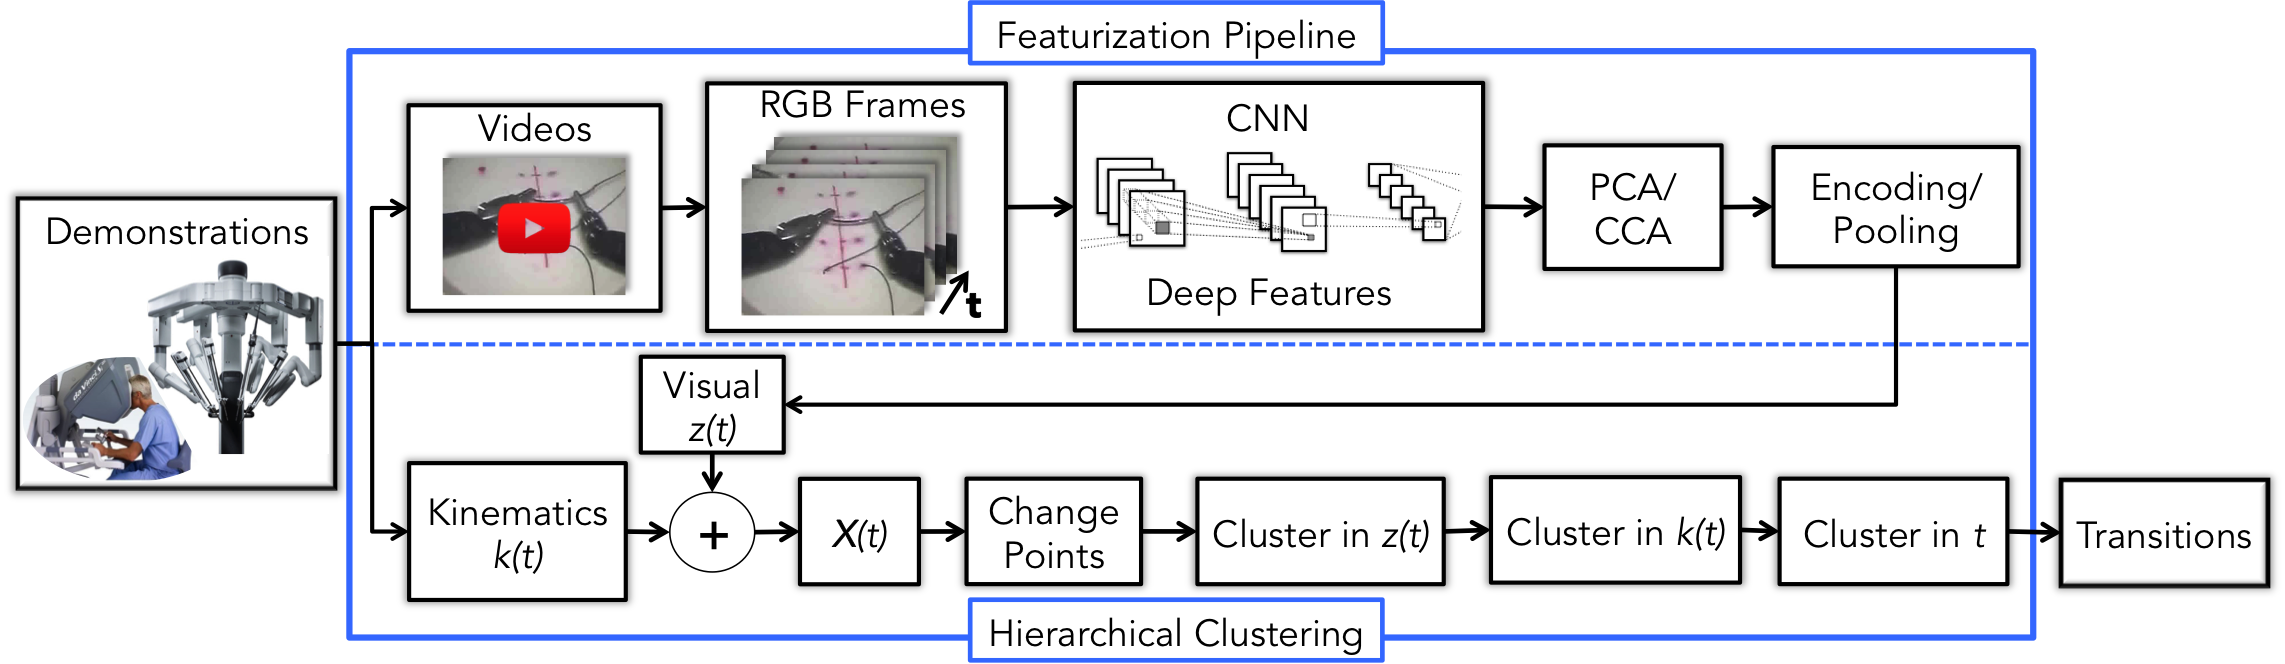
\includegraphics[width=1.55\linewidth]{figures/sysArch}
    \caption{We use a visual processing pipeline with deep features to construct a trajectory of high-dimensional visual states $z(t)$.
    We concatenate encoded versions of these features with kinematics and apply hierarchical clustering to find segments.}%dont add more lines--seems to mess up formatting
    \label{fig:pipeline}
    \vspace{-10pt}
\end{SCfigure*}
\fi
% \fi

% \begin{figure*}[!t]
% \centering
% 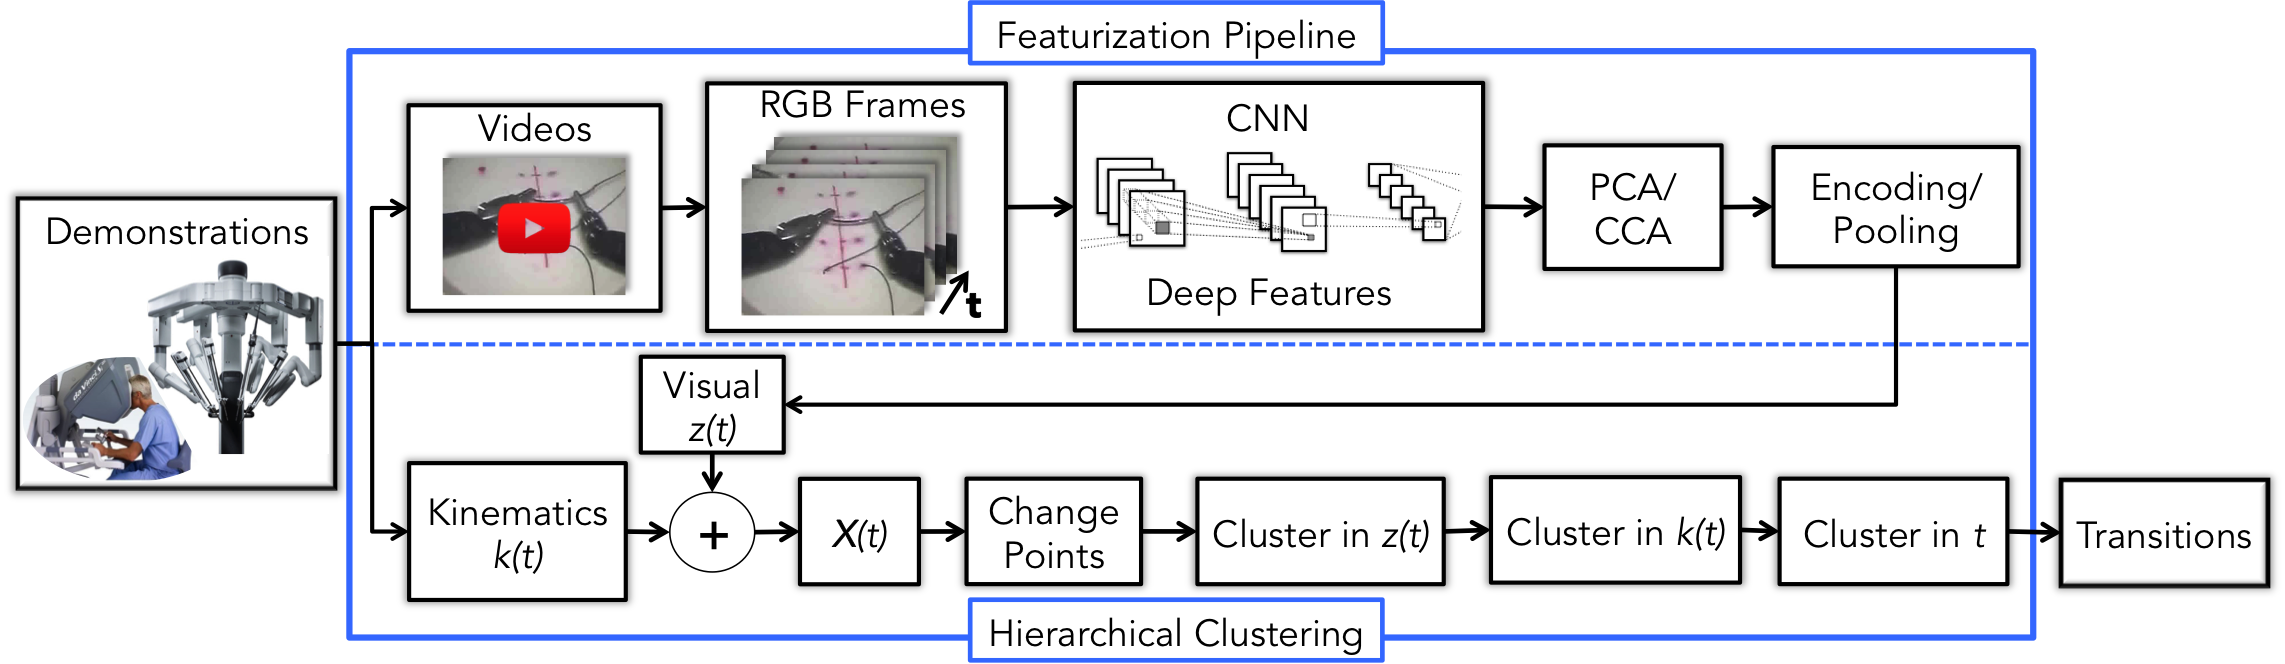
\includegraphics[width=0.8\linewidth]{figures/sysArch}
% \caption{\tsc is a task segmentation pipeline that starts with multimodal demonstrations (kinematics and vision), uses deep learning to featurize the frames of the video, and then clusters transition events to find segments.}
% \label{fig:pipeline}
% \vspace{-15pt}
% \end{figure*}


We evaluate \tsc on three datasets: (1) a synthetic 4 segment example, (2) JIGSAWS surgical needle passing,  and (3) JIGSAWS surgical suturing.
On the synthetic example, we find that \tsc recovers the 4 underlying segments in the presence of partial state observation (one kinematic state hidden), control noise, and sensor noise. 
We also compare \tsc with manual annotations when available.
On real datasets, we find that \tsc matches the manual annotation with up to 0.806 normalized mutual information.
Our results also suggest that including kinematics and vision results in increases of up-to 0.215 NMI over kinematics alone.
We demonstrate the benefits of using an unsupervised approach by presenting examples where \tsc discovers unlabeled segments due to human annotator error (as shown in Figure \ref{fig:suturing}), and can learn across demonstrations with widely varying operator skill levels (as shown in Table \ref{tab:jigsaws}).


%Clustering allows focussed LFD on each segment resulting in a better fit. 
%Clustering can identify inconsistent outliers and dirty data segments that cann corrupt LFD, also 
%Can identify segments where more consistent data is needed.
%can salvage good segments form bad demo sequences. 

%emph unsupervised
%avoids human bias
%apply consistent models -- can discover subtle transitions
%faster than humans 
  
\iffalse
\begin{figure}[ht]
\centering
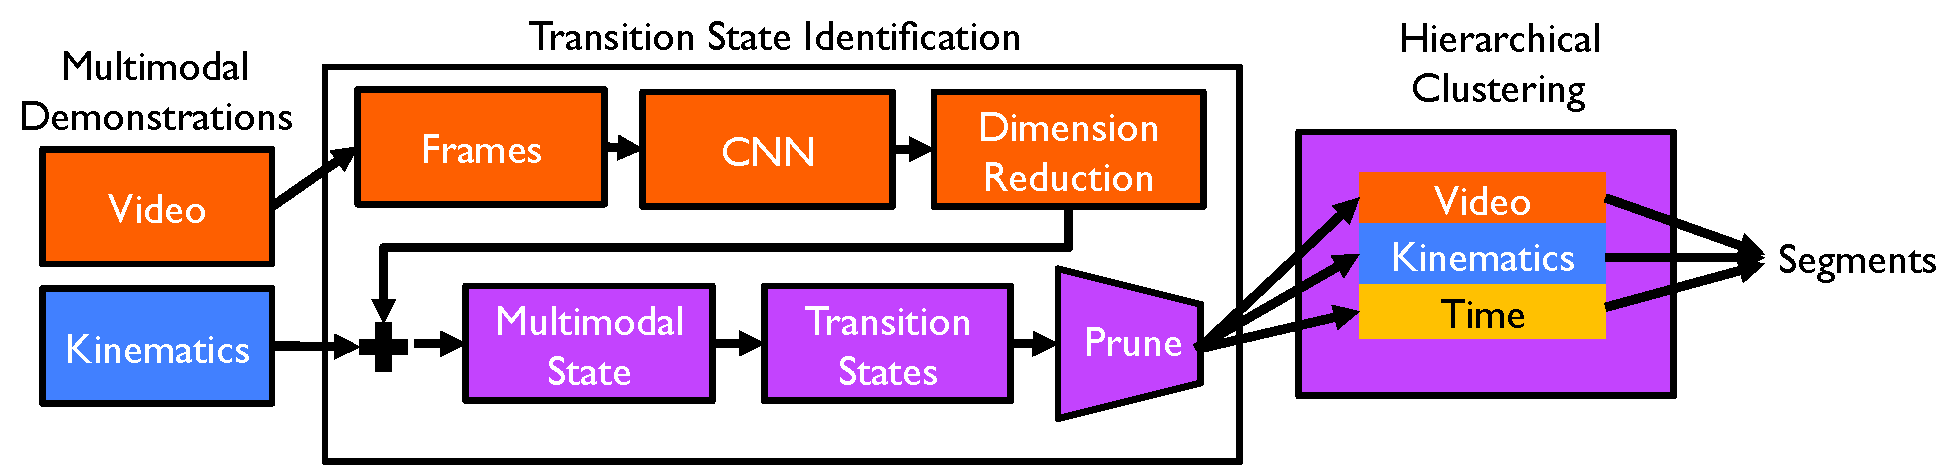
\includegraphics[width=\columnwidth]{figures/architecture.pdf}
\caption{\todo{name} architecture. We use a pre-trained CNN to featurize raw video data for use in segmentation. After featurization, we combine the data with kinematic data and apply a Transition State Clustering algorithm to identify segments.}
\figlabel{arch}
\vspace{-1em}
\end{figure}
\fi

\end{document}